\documentclass[a4paper,9pt]{extarticle}

\usepackage{amsfonts, amsmath, amssymb, amsthm, enumitem, fancyhdr, graphicx}
\usepackage[margin=0.5in, includehead, includefoot, heightrounded]{geometry}
\allowdisplaybreaks
\pagestyle{fancy}
\rhead{Erick Lin}

\newcommand*\dist{\mathop{\!\mathrm{d}}}
\newcommand{\norm}[1]{\left\lVert#1\right\rVert}
\renewcommand{\thesubsection}{\arabic{subsection}}
\DeclareMathOperator*{\argmax}{\arg\!\max}
\DeclareMathOperator*{\argmin}{\arg\!\min}
\DeclareMathOperator*{\vol}{vol}
\DeclareMathOperator*{\esssup}{ess\,sup}
\DeclareMathOperator*{\BV}{BV}
\DeclareMathOperator*{\Lip}{Lip}
\DeclareMathOperator*{\AC}{AC}
\theoremstyle{definition}
\newtheorem{defin}{Definition}
\newtheorem{thm}{Theorem}
\newtheorem{lem}[thm]{Lemma}
\newtheorem{cor}[thm]{Corollary}

\begin{document}

\sloppy
\begin{lem}
    If $U$ is a nonempty open subset of $\mathbb{R}^d$, then there exist countably many nonoverlapping cubes $\{Q_k\}_{k \in \mathbb{N}}$ such that $U = \bigcup Q_k$.
\end{lem}
\iffalse
    \begin{lem}
        Let $Q = \prod_{j = 1}^d [a_j, b_j]$ be a box in $\mathbb{R}^d$. If $Q_1, \cdots, Q_n$ are nonoverlapping boxes such that $Q = Q_1 \cup \cdots \cup Q_n$, then
        \begin{align*}
            \vol(Q) = \sum_{k = 1}^n \vol(Q_k).
        \end{align*}
    \end{lem}
\fi
\begin{defin}
    If $\{ E_k \}_{k \in \mathbb{N}}$ is a sequence of subsets of $\mathbb{R}^d$, then we set
    \begin{align*}
        \limsup_{k \to \infty} E_k = \bigcap_{j = 1}^\infty \bigcup_{k = j}^\infty E_k
        \qquad \text{and} \qquad
        \liminf_{k \to \infty} E_k = \bigcup_{j = 1}^\infty \bigcap_{k = j}^\infty E_k.
    \end{align*}
\end{defin}
\begin{thm}[Regularity]
    Given $E \subseteq \mathbb{R}^d$ and $\varepsilon > 0$, there exists an open set $U \supseteq E$ such that
    \begin{align*}
        |E|_e \leq |U|_e \leq |E|_e + \varepsilon.
    \end{align*}
    (If $|E|_e < \infty$, then the inequality on the right is strict.) Consequently,
    \begin{align*}
        |E|_e = \inf\{ |U|_e : U \text{ open}, U \supseteq E \}.
    \end{align*}
\end{thm}
\begin{defin}[Lebesgue Measure]
    A set $E \subseteq \mathbb{R}^d$ is \emph{(Lebesgue) measurable} if
    \begin{align*}
        \forall\; \varepsilon > 0, \quad \exists \text{ open } U \supseteq E \text{ such that } |U \setminus E|_e \leq \varepsilon.
    \end{align*}
\end{defin}
\begin{thm}
    $\mathcal{L}$ is closed under countable unions and complements. In other words, $\mathcal{L}$ is a \emph{$\sigma$-algebra}.
\end{thm}
\begin{cor}
    $\mathcal{L}$ is closed under countable intersections and \emph{relative complements} --- in other words, if $A$ and $B$ are measurable subsets of $\mathbb{R}^d$, then so is $A \setminus B$.
\end{cor}
\begin{lem}
    A set $E \subseteq \mathbb{R}^d$ is measurable if and only if for each $\varepsilon > 0$ there exists a closed set $F \subseteq E$ such that $|E \setminus F|_e \leq \varepsilon$.
\end{lem}
\begin{thm}[Countable Additivity]
    If $E_1, E_2, \cdots$ are disjoint, measurable subsets of $\mathbb{R}^d$, then
    \begin{align*}
        \left| \bigcup_{k = 1}^\infty E_k \right| = \sum_{k = 1}^\infty |E_k|.
    \end{align*}
\end{thm}
\begin{defin}
    A set $H \subseteq \mathbb{R}^d$ is
    \begin{itemize}[itemsep=0ex]
        \item
            a $G_\delta$-set if there exist countably many open sets $U_k$ such that $H = \bigcap U_k$.
        \item
            an $F_\sigma$-set if there exist countably many closed sets $F_k$ such that $H = \bigcup F_k$.
    \end{itemize}
\end{defin}
\begin{lem}
    Given a set $E \subseteq R^d$, TFAE:
    \begin{itemize}[itemsep=0ex]
        \item
            $E$ is measurable.
        \item
            $E = H \setminus Z$ where $H$ is a $G_\delta$-set and $|Z| = 0$.
        \item
            $E = H \cup Z$ where $H$ is a $F_\sigma$-set and $|Z| = 0$.
    \end{itemize}
\end{lem}
\begin{thm}[Carath\'eodory's Criterion]
    A set $E \subseteq \mathbb{R}^d$ is measurable if and only if
    \begin{align*}
        \forall\; A \subseteq \mathbb{R}^d, \quad |A|_e = |A \cap E|_e + |A \setminus E|_e.
    \end{align*}
\end{thm}
\begin{lem}
    If $A \subseteq B$ are measurable sets and $|A| < \infty$ then
    \begin{align*}
        |B \setminus A| = |B| - |A|.
    \end{align*}
\end{lem}
\iffalse
    \begin{lem}[Continuity from Below]
        If $E_1 \subseteq E_2 \subseteq \cdots$ are measurable subsets of $\mathbb{R}^d$, then $|E_1| \leq |E_2| \leq \cdots$ and
        \begin{align*}
            \left| \bigcup_{k = 1}^\infty E_k \right| = \lim_{k \to \infty} |E_k|.
        \end{align*}
    \end{lem}
\fi
\begin{lem}[Continuity from Above]
    If $E_1 \supseteq E_2 \supseteq \cdots$ are measurable subsets of $\mathbb{R}^d$ and $|E_k| < \infty$ for some $k$, then $|E_1| \geq |E_2| \geq \cdots$ and
    \begin{align*}
        \left| \bigcap_{k = 1}^\infty E_k \right| = \lim_{k \to \infty} |E_k|.
    \end{align*}
\end{lem}
\begin{cor}
    If $E \subseteq \mathbb{R}^d$ is measurable and $|E| < \infty$, then there exist open sets $V_1 \supseteq V_2 \supseteq \cdots \supseteq E$ such that $\lim_{k \to \infty} |V_k| = |E|$.
\end{cor}
\begin{lem}
    Let $E \subseteq \mathbb{R}^d$ be a measurable set, and let $f : E \to \mathbb{F}$ be a measurable function. If $g : E \to \mathbb{F}$ satisfies $g = f$ a.e., then $g$ is measurable.
\end{lem}
\iffalse
\begin{thm}
    Let $E \subseteq \mathbb{R}^d$ be a measurable set, and let $f : E \to [0, \infty]$ be a nonnegative, measurable function on $E$.
    \begin{enumerate}[label=(\alph*)]
        \item
            There exist nonnegative simple functions $\phi_n$ such that $\phi_n \nearrow f$.
        \item
            If $f$ is bounded on some set $A \subseteq E$, then we can construct the functions $\phi_n$ in statement (a) so that they converge uniformly to $f$ on $A$.
    \end{enumerate}
\end{thm}
\fi
\begin{thm}
    Let $E \subseteq \mathbb{R}^d$ be a measurable set, and let $f : E \to \mathbb{F}$ be a measurable function on $E$. Then there exist simple functions $\phi_n$ on $E$ such that:
    \begin{enumerate}[itemsep=0ex, label=(\alph*)]
        \item
            $\lim_{n \to \infty} \phi_n(x) = f(x)$ for every $x \in E$,
        \item
            $|\phi_n(x)| \leq |f(x)|$ for every $n \in \mathbb{N}$ and $x \in E$,
        \item
            the convergence is uniform on every set on which $f$ is bounded.
    \end{enumerate}
\end{thm}
\begin{defin}
    The \emph{Lebesgue space of essentially bounded functions on $E$} is
    \begin{align*}
        L^\infty(E) = \left\{ f : E \to \mathbb{F} : f \text{ is measurable and } \norm{f}_\infty = \esssup_{x \in E} |f(x)| < \infty \right\}.
    \end{align*}
\end{defin}
\begin{lem}
    If $E$ is a measurable subset of $\mathbb{R}^d$, then any Cauchy sequence converges in $L^\infty$-norm, i.e., $L^\infty(E)$ is complete.
\end{lem}
\begin{thm}[Egorov]
    Let $E \subseteq \mathbb{R}^d$ be a measurable set such that $|E| < \infty$. Suppose that $\{f_n\}_{n \in \mathbb{N}}$ is a sequence of measurable functions $E \to \mathbb{F}$ and $f_n \to f$ a.e. where $f$ is finite a.e. Then $f_n \to f$ \emph{almost uniformly}, i.e., for each $\varepsilon > 0$ there exists a measurable set $A \subseteq E$ such that $|A| < \varepsilon$ and $f_n \to f$ uniformly on $E \setminus A$.
\end{thm}
\begin{defin}
    Let $E \subseteq \mathbb{R}^d$ be a measurable set, and let $f_n, f$ be measurable functions on $E$ that are either complex-valued or extended real-valued but finite a.e. Then $f_n \xrightarrow{m} f$ if
    \begin{align*}
        \forall\; \varepsilon > 0, \quad \lim_{n \to \infty} |\{|f - f_n| > \varepsilon \}| = 0.
    \end{align*}
\end{defin}
\begin{thm}
    Let $E \subseteq \mathbb{R}^d$ be a measurable set. If $\{f_n\}_{n \in \mathbb{N}}$ is a sequence of measurable functions that is Cauchy in measure on $E$, then there exists a measurable function $f$ such that $f_n \xrightarrow{m} f$.
\end{thm}
\begin{thm}[Luzin]
    Let $E$ be a bounded, measurable subset of $\mathbb{R}^d$, and let $f : E \to \mathbb{F}$ be measurable and finite a.e. Then for each $\varepsilon > 0$, there exists a closed set $F \subseteq E$ such that $|E \setminus F| < \varepsilon$ and $f|_F$ is continuous.
\end{thm}
\begin{thm}[Tchebyshev's Inequality]
    Let $f : E \to [0, \infty]$ be a measurable, nonnegative function defined on a measurable set $E \subseteq \mathbb{R}^d$. Then for each number $\alpha > 0$ we have
    \begin{align*}
        |\{ f > \alpha \}| \leq \frac{1}{\alpha} \int_{\{f > \alpha\}} f \leq \frac{1}{\alpha} \int_E f.
    \end{align*}
\end{thm}
\begin{thm}[Monotone Convergence]
    Let $E \subseteq \mathbb{R}^d$ be a measurable set, and let $f_n : E \to [0, \infty]$ be nonnegative a.e., measurable functions on $E$ such that $f_n \nearrow f$. Then
    \begin{align*}
        \lim_{n \to \infty} \int_E f_n = \int_E f.
    \end{align*}
\end{thm}
\begin{thm}[Fatou's Lemma]
    If $\{f_n\}_{n \in \mathbb{N}}$ is a sequence of measurable, nonnegative a.e., extended real-valued functions on a measurable set $E \subseteq \mathbb{R}^d$, then
    \begin{align*}
        \int_E \left( \liminf_{n \to \infty} f_n \right) \leq \liminf_{n \to \infty} \int_E f_n.
    \end{align*}
    In particular, if $f_n \to f$ pointwise, then
    \begin{align*}
        \int_E f \leq \liminf_{n \to \infty} \int_E f_n.
    \end{align*}
\end{thm}
\begin{defin}
    The \emph{Lebesgue space of integrable functions on $E$} is
    \begin{align*}
        L^1(E) = \left\{ f : E \to \mathbb{F} : f \text{ is measurable and } \norm{f}_1 = \int_E |f| < \infty \right\}.
    \end{align*}
\end{defin}
\begin{center}
    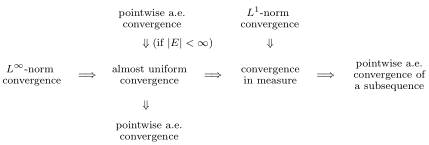
\includegraphics{convergence_relations}
\end{center}
\begin{thm}[Dominated Convergence]
    Let $\{f_n\}_{n \in \mathbb{N}}$ be a sequence of measurable functions $E \to \mathbb{F}$ where $E \subseteq \mathbb{R}^d$. If
    \begin{enumerate}[itemsep=0ex, label=(\alph*)]
        \item
            $f(x) = \limsup_{n \to \infty} f_n(x)$ exists for a.e. $x \in E$, and
        \item
            there exists $g \in L^1(E)$ such that for each $n \in \mathbb{N}$ we have $|f_n(x)| \leq g(x)$ a.e.,
    \end{enumerate}
    then $f_n \to f$ in $L^1$-norm.
\end{thm}
\begin{thm}
    If $f \in L^1(\mathbb{R}^d)$ and $\varepsilon > 0$, then there exists $\theta \in C_c(\mathbb{R}^d)$ such that $\norm{f - \theta}_1 < \varepsilon$.
\end{thm}
\begin{cor}[Strong Continuity of Translation on $L^1(\mathbb{R}^d)$]
    Given $f \in L^1(\mathbb{R}^d)$, let $T_a f(x) = f(x - a)$ denote the translation of $f$ by $a \in \mathbb{R}^d$. Then $T_a f \to f$ in $L^1$-norm as $a \to 0$.
\end{cor}
\begin{thm}
    If $f \in L^1(\mathbb{R})$, then for each $\varepsilon > 0$ there exists a really simple function $\phi$ such that $\norm{f - \phi}_1 < \varepsilon$.
\end{thm}
\textbf{Fubini's} and \textbf{Tonelli's Theorems} apply when given $E \subseteq \mathbb{R}^m, F \subseteq \mathbb{R}^n$ measurable, $f : E \times F \to \mathbb{F}$ is integrable/measurable.
\begin{thm}[Convolution is Submultiplicative]
    If $f, g \in L^1(\mathbb{R}^d)$, then $f * g \in L^1(\mathbb{R}^d)$ and
    \begin{align*}
        \norm{f * g}_1 \leq \norm{f}_1 \norm{g}_1.
    \end{align*}
\end{thm}
\begin{defin}[Bounded Variation]
    Let $f: [a, b] \to \mathbb{C}$ be given. For each finite partition $\Gamma = \{ a = x_0 < \cdots < x_n = b \}$ of $[a, b]$, set
    \begin{align*}
        S_\Gamma = S_\Gamma[f; a, b] = \sum_{j = 1}^n |f(x_j) - f(x_{j - 1})|.
    \end{align*}
    The \emph{total variation of $f$} over $[a, b]$ is
    \begin{align*}
        V[f; a, b] = \sup\{ S_\Gamma : \Gamma \text{ is a partition of } [a, b] \}.
    \end{align*}
    Then $f$ has \emph{bounded variation} on $[a, b]$ (i.e., $f \in \BV[a, b]$) if $V[f; a, b] < \infty$.
\end{defin}
$C^1[a, b] \subsetneq \Lip[a, b] \subsetneq \BV[a, b]$.
\begin{lem}
    If $g \in L^1[a, b]$, then given its indefinite integral
    \begin{align*}
        G(x) = \int_a^x g(t) dt, \qquad x \in [a, b],
    \end{align*}
    \begin{enumerate}[itemsep=0ex, label=(\alph*)]
        \item
            $G$ is continuous on $[a, b]$,
        \item
            $G \in \BV[a, b]$,
        \item
            the total variation of $G$ is bounded by the $L^1$-norm of $g$, i.e.,
            \begin{align*}
                V[G; a, b] \leq \int_a^b |g(t)| dt = \norm{g}_1.
            \end{align*}
    \end{enumerate}
\end{lem}
\begin{thm}
    Given $f : [a, b] \to \mathbb{R}$, $f \in \BV[a, b]$ if and only if there exist monotone increasing functions $g, h$ such that $f = g - h$.
\end{thm}
\begin{thm}[Simple Vitali Lemma]
    Let $\mathcal{B}$ be any collection of open balls in $\mathbb{R}^d$. Let $U$ be the union of all the balls in $\mathcal{B}$, and fix $0 < c < |U|$. Then there exist finitely many disjoint balls $B_1, \cdots, B_N \in \mathcal{B}$ such that
    \begin{align*}
        \sum_{k = 1}^N |B_k| > \frac{c}{3^d}.
    \end{align*}
\end{thm}
\begin{defin}
    A collection $\mathcal{B}$ of closed balls is a \emph{Vitali cover} of a set $E \subseteq \mathbb{R}^d$ if for each $x \in E$ and $\varepsilon > 0$ there exists some ball $B \in \mathcal{B}$ such that $x \in B$ and $\text{radius}(B) < \varepsilon$.
\end{defin}
\begin{thm}[Vitali Covering Lemma]
    Let $E$ be a subset of $\mathbb{R}^d$ with $0 < |E|_e < \infty$. If $\mathcal{B}$ is a Vitali covering of $E$, then for each $\varepsilon > 0$ there exist disjoint balls $B_1, \cdots, B_N \in \mathcal{B}$ such that
    \begin{align*}
        \left| E \setminus \bigcup_{k = 1}^N B_k \right| < \varepsilon
        \qquad \text{and} \qquad
        \sum_{k = 1}^N |B_k| < |E|_e + \varepsilon.
    \end{align*}
\end{thm}
\begin{thm}
    Monotone functions are differentiable a.e., so for any $f \in \BV[a, b]$, the $L^1$-norm of $f'$ is bounded by the total variation of $f$. Also, any convergent series of monotone increasing functions is differentiable a.e.
\end{thm}
\begin{lem} \label{lem:pre-diff}
    If a function $f : \mathbb{R}^d \to \mathbb{C}$ is continuous at a point $x \in \mathbb{R}^d$, then
    \begin{gather*}
        \lim_{h \to 0} \frac{1}{|B_h(x)|} \int_{B_h(x)} |f(x) - f(t)| dt = 0 \\
        \lim_{h \to 0} \tilde{f_h}(x) = \lim_{h \to 0} \frac{1}{|B_h(x)|} \int_{B_h(x)} f(t) dt = f(x).
    \end{gather*}
\end{lem}
\begin{thm}
    If $f \in L^1(\mathbb{R}^d)$, then $\tilde{f_h} \to f$ in $L^1$-norm.
\end{thm}
\begin{defin}
    A measurable function $f : \mathbb{R}^d \to \mathbb{F}$ is \emph{locally integrable} if its restriction to any compact set $K$ is integrable. Then the \emph{Hardy-Littlewood maximal function} of $f$ is
    \begin{align*}
        Mf(x) = \sup_{h > 0} \tilde{f_h}(x) = \sup_{h > 0} \frac{1}{|B_h(x)|} \int_{B_h(x)} |f(t)| dt.
    \end{align*}
\end{defin}
\begin{thm}[Maximal]
    If $f \in L^1(\mathbb{R}^d)$, then for each $\alpha > 0$ we have
    \begin{align*}
        |\{ Mf > \alpha \}| \leq \frac{3^d}{\alpha} \int_{\mathbb{R}^d} |f| = \frac{3^d}{\alpha} \norm{f}_1.
    \end{align*}
\end{thm}
\begin{thm}[Lebesgue's Differentiation]
    Lemma \ref{lem:pre-diff}, but with the hypotheses that $f$ is locally integrable and for a.e. $x \in \mathbb{R}^d$.
\end{thm}
\begin{thm}
    If $f$ is locally integrable on $\mathbb{R}^d$ and $\{ E_n \}_{n \in \mathbb{N}}$ shrinks regularly to a Lebesgue point $x$ of $f$, then
    \begin{align*}
        \lim_{n \to \infty} \frac{1}{|E_n|} \int_{E_n} |f(x) - f(t)| dt = 0.
    \end{align*}
\end{thm}
\begin{defin}
    A function $f : [a, b] \to \mathbb{C}$ is \emph{absolutely continuous on $[a, b]$}, i.e. $f \in \AC[a, b]$, if for every $\varepsilon > 0$ there exists $\delta > 0$ such that for any countable collection of nonoverlapping subintervals $\{[a_j, b_j]\}$ of $[a, b]$, we have
\end{defin}
\begin{align*}
    \sum_j (b_j - a_j) < \delta
    \quad \Longrightarrow \quad
    \sum_j |f(b_j) - f(a_j)| < \varepsilon.
\end{align*}
\begin{lem}
    $C^1[a, b] \subsetneq \Lip[a, b] \subsetneq \AC[a, b] \subsetneq \BV[a, b] \subsetneq L^\infty[a, b] \subsetneq L^1[a, b]$.
\end{lem}
\begin{cor}
    If $f \in \AC[a, b]$, then $f'(x)$ exists for a.e. $x$, and $f' \in L^1[a, b]$. The Banach-Zaretsky Theorem implies that the converse is also true.
\end{cor}
\begin{lem}
    If $g \in L^1[a, b]$, then its indefinite integral $G$ is absolutely continuous on $[a, b]$, differentiable a.e., and satisfies $G' \in L^1[a, b]$.
\end{lem}
\begin{lem}
    If $f : [a, b] \to \mathbb{C}$ is both absolutely continuous and singular, then $f$ is constant.
\end{lem}
\begin{lem}
    If $g \in L^1[a, b]$, then its indefinite integral $G$ is absolutely continuous and satisfies $G' = g$ a.e.
\end{lem}
\begin{thm}[Fundamental Theorem of Calculus]
    Given a function $f : [a, b] \to \mathbb{C}$, TFAE:
    \begin{enumerate}[itemsep=0ex]
        \item
            $f \in \AC[a, b].$
        \item
            There exists a function $g \in L^1[a, b]$ such that
            \begin{align*}
                f(x) - f(a) = \int_a^x g(t) dt, \qquad x \in [a, b].
            \end{align*}
        \item
            $f$ is differentiable a.e. on $[a, b]$, $f' \in L^1[a, b]$, and
            \begin{align*}
                f(x) - f(a) = \int_a^x f(t) dt, \qquad x \in [a, b].
            \end{align*}
    \end{enumerate}
\end{thm}
\begin{cor}
    If $f \in \BV[a, b]$, then $f = g + h$ where $g \in \AC[a, b]$ and $h$ is singular on $[a, b]$. Moreover, $g$ and $h$ are unique up to an additive constant, and we can take
    \begin{align*}
        g(x) = \int_a^x f'(t) dt, \qquad x \in [a, b].
    \end{align*}
\end{cor}
\begin{thm}
    If $f \in \AC[a, b]$, then $V[f; a, b] = \int_a^b |f'|$.
\end{thm}
\begin{cor}
    Given $f \in \AC[a, b]$, then $V \in \AC[a, b]$, $V(x) = \int_a^x |f'|$ for each $x \in [a, b]$, and $V' = |f'|$ a.e.
\end{cor}
\begin{thm}[Integration by Parts]
    If $f, g \in \AC[a, b]$, then
    \begin{align*}
        \int_a^b f(x) g'(x) dx = f(b)g(b) - f(a)g(a) - \int_a^b f'(x)g(x)dx.
    \end{align*}
\end{thm}
\begin{thm}
    If $f \in L^1[a, b]$ satisfies
    \begin{align*}
        \int_a^b f(x)g(x)dx = 0 \qquad \text{for all} \qquad g \in C[a, b],
    \end{align*}
    then $f = 0$ a.e.
\end{thm}
\begin{defin}
    Given $-\infty \leq a < b \leq \infty$, a function $\phi : (a, b) \to \mathbb{R}$ is \emph{convex} on the open interval $(a, b)$ if for all $x, y \in (a, b)$ and $0 < t < 1$ we have
    \begin{align*}
        \phi(tx + (1 - t)y) \leq t\phi(x) + (1 - t)\phi(y).
    \end{align*}
\end{defin}
\begin{thm}[Jensen's Inequality]
    Let $E$ be a measurable subset of $\mathbb{R}^d$ such that $0 < |E| < \infty$. If $g : E \to (a, b)$ is integrable and $\phi$ is convex on $(a, b)$, then
    \begin{align*}
        \phi\left( \frac{1}{|E|} \int_E g \right) \leq \frac{1}{|E|} \int_E \phi \circ g.
    \end{align*}
\end{thm}
\begin{thm}[H\"older's Inequality]
    Fix $1 \leq p \leq \infty$ and let $p'$ be the dual index to $p$. If $x = (x_k)_{k \in \mathbb{N}} \in \ell^p$ and $y = (y_k)_{k \in \mathbb{N}} \in \ell^{p'}$, then the sequence $xy = (x_k y_k)_{k \in \mathbb{N}} \in \ell^1$, and
    \begin{align*}
        \norm{xy}_1 \leq \norm{x}_p \norm{y}_{p'}.
    \end{align*}
\end{thm}
\begin{thm}[Minkowski's Inequality]
    Fix $1 < p < \infty$. If $x, y \in \ell^p$, then
    \begin{align*}
        \norm{x + y}_p \leq \norm{x}_p + \norm{y}_p.
    \end{align*}
\end{thm}
\begin{thm}[Converse of H\"older's Inequality]
    Let $E$ be measurable subset of $\mathbb{R}^d$, and fix $1 \leq p \leq \infty$. Then for each function $f \in L^p(E)$ we have
    \begin{align*}
        \sup_{\norm{g}_{p'} = 1} \left| \int_E fg \right| = \norm{f}_p.
    \end{align*}
    Furthermore, there exists a function $g \in L^{p'}(E)$ such that $\norm{g}_{p'} = 1$ and $\int_E fg = \norm{f}_p$.
\end{thm}
\begin{thm}
    Let $E \subseteq \mathbb{R}^d$ be a measurable set. If $1 \leq p < \infty$, then $L_c^p(E)$ is dense in $L^p(E)$.
\end{thm}

\end{document}
